\documentclass[10pt]{beamer}

\usepackage{cmap}%allows cyrillic search in pdf
\usepackage[english,russian,ukrainian]{babel}
\usepackage[T2A]{fontenc}
\usepackage[utf8]{inputenc}

\usetheme[progressbar=frametitle]{metropolis}
\usepackage{appendixnumberbeamer}

\usepackage{booktabs}
%\usepackage[scale=2]{ccicons}

%\usepackage{pgfplots}
%\usepgfplotslibrary{dateplot}

%\usepackage{xspace}
%\newcommand{\themename}{\textbf{\textsc{metropolis}}\xspace}

\usepackage{wrapfig,graphicx,caption,subcaption,overpic}
\usepackage{amsmath, amssymb, amsfonts}
\usefonttheme[onlymath]{serif}
\usepackage{xcolor}

\title{ЕЛЕКТРОФІЗИЧНІ ВЛАСТИВОСТІ\\ БАГАТОФАЗНИХ ДИСПЕРСНИХ СИСТЕМ}
%\subtitle{A modern beamer theme}
% \date{\today}
\date{}
\author{Семенов Андрій Костянтинович}
\institute{Науковий керівник: к.ф.-м.н., доц. М. Я. Сушко\\
Кафедра теоретичної фізики та астрономії\\
Одеський національний університет імені І.І. Мечникова}
% \titlegraphic{\hfill\includegraphics[height=1.5cm]{logo.pdf}}

\begin{document}

\maketitle

%%%%%%%%%%%%%%%%%%%%%%%%%%%%%%%%%%%%%%%%%%%%%%%%%%%%%%
\begin{frame}{Мета роботи та поставлені задачі}

{\bf Мета роботи}:

{\footnotesize 
Побудова самоузгодженої макроскопічної теорії довгохвильового електричного відгуку немагнітних макроскопічно однорідних та ізотропних дисперсних систем.
}

{\bf Задачі}:

{\footnotesize 
--- Узагальнити метод компактних груп (МКГ) на випадок провідних систем.

--- Розробити послідовний метод електричної гомогенізації макроскопічно однорідних та ізотропних систем в рамках МКГ.

--- Побудувати модель дисперсної системи сферичних частинок з морфологією типу тверде ядро--проникна оболонка.

--- Протестувати адекватність розробленої теорії на числових даних.

--- Проаналізувати характеристики перколяційної поведінки провідності та проникності в рамках теорії.

--- Застосувати теоретичні результати до обробки експериментальних даних.

}

\end{frame}

%%%%%%%%%%%%%%%%%%%%%%%%%%%%%%%%%%%%%%%%%%%%%%%%%%%%%%
\begin{frame}{Публікації}

  \begin{itemize}
    \item
    Sushko M. Ya. Conductivity and permittivity of dispersed systems 
    with penetrable particle-host interphase~/ M.~Ya.~Sushko, 
    A.~K.~Semenov~// Cond. Matter Phys. --- 2013 --- Vol.~16 --- No. 1 
    --- P.~13401.
    
    \item
    Semenov~A.~K. On applicability of differential mixing rules for
      statistically homogeneous and isotropic dispersions~/ A.~K.~Semenov~//
      J. Phys. Commun. --- 2018. --- Vol.~2. --- No. 3 --- P.~035045.
    
    \item
    Sushko~M.~Ya. A mesoscopic model for the effective electrical 
    conductivity of composite polymeric electrolytes.~/ M.~Ya.~Sushko,
    A.~K.~Semenov~// J. Mol. Liq. --- 2019. --- Vol.~279 --- P.~677.
    
    \item
    Sushko~M.~Ya. Rigorously solvable model for the electrical conductivity of dispersions of hard-core--penetrable-shell particles and its applications~/
    M.~Ya.~Su\-shko, A.~K.~Semenov~//
    Phys. Rev. E --- 2019. --- Vol.~100. --- P.~052601.
  \end{itemize}

\end{frame}

%%%%%%%%%%%%%%%%%%%%%%%%%%%%%%%%%%%%%%%%%%%%%%%%%%%%%%
\begin{frame}{Участь у міжнародних конференціях та семінарах}
\vspace{-5pt}
{\footnotesize
\begin{enumerate}
\item 4-th International Conference on Statistical
Physics: Modern Trends and Applications, Lviv (Ukraine), 2012.

\item 25-th International
Conference: Disperse Systems, Odesa (Ukraine), 2012.

\item 5-th International Symposium: Methods and
Applications of Computational Chemistry,  Kharkiv (Ukraine), 2013.

\item 6-th International
Conference Physics  of  Liquid  Matter:  Modern Problems,
 Kyiv (Ukraine), 2014.

\item 26-th International
Conference: Disperse Systems,  Odesa (Ukraine), 2014.

\item 2015 International Young
Scientists Forum on Applied Physics,  Dnipropetrovsk (Ukraine), 2015.

\item 27-th International
Conference: Disperse Systems, Odesa (Ukraine), 2016.

\item International conference: Development of innovation in the
technical, physical and mathematical fields of sciences, Mykolayiv (Ukraine), 2016.

\item 8-th International  Conference Physics  of  Liquid  Matter:
Modern Problems, Kyiv (Ukraine), 2018.

\item 5-th International Conference on Statistical
Physics: Modern Trends and Applications, Lviv (Ukraine), 2019.

\item 7-th International Conference: Nano\-technologies 
and Nanomaterials,  Lviv (Ukraine), 2019.

\item 28-th International
Conference: Disperse Systems, Odesa (Ukraine), 2019.
\end{enumerate}
}

\end{frame}


%%%%%%%%%%%%%%%%%%%%%%%%%%%%%%%%%%%%%%%%%%%%%%%%%%%%%%
\begin{frame}{Актуальність роботи}

  \begin{itemize}
    \item Дисперсні системи широко використовуються в промисловості.
    \item Передбачення їх електричних властивостей грає значну роль при створенні нових композитних матеріалів.
    \item Не існує єдиної самоузгодженої багаточастинкової теорії електричного відгуку таких систем.
    \item Не існує чіткого розмежування між типами систем при застосуванні симетричного та асиметричного (диференціального) підходів моделювання.
  \end{itemize}

\end{frame}

%%%%%%%%%%%%%%%%%%%%%%%%%%%%%%%%%%%%%%%%%%%%%%%%%%%%%%
\begin{frame}{План доповіді}
  \footnotesize
  \setbeamertemplate{section in toc}[sections numbered]
  \tableofcontents%[hideallsubsections]
  \vspace{-25pt}
\end{frame}


%%%%%%%%%%%%%%%%%%%%%%%%%%%%%%%%%%%%%%%%%%%%%%%%%%%%%
\section[Вступ]{Вступ}%%%%%%%%%%%%%%%%%%%%%%%%%%%%%%%
%%%%%%%%%%%%%%%%%%%%%%%%%%%%%%%%%%%%%%%%%%%%%%%%%%%%%
\subsection{Типи дисперсних систем, що розглядаються, та їх особливості}

\begin{frame}{Тверді композитні електроліти}
\footnotesize
\footnotesize

%(Високопровідна оболонка, менш провідні ядро та матриця: $\sigma_2 \gg \sigma_1, \sigma_0$)
\vspace{5pt}

\begin{wrapfigure}{r}{0.4\textwidth}
\vspace{-25pt}
  \begin{center}
    \begin{overpic}[width=0.45\textwidth]{images/liang.eps}
         \put(60,15){$\rm LiI-Al_2O_3$}
    \end{overpic}
  \end{center}
\vspace{-50pt}
\end{wrapfigure}

---~Матриця: (полі)кристалічні галоїди металів (наприклад, літію, срібла, міді)\vspace{5pt}

--- Дисперсна фаза:  низькопровідні частинки (наприклад, оксид алюмінія).\vspace{5pt}

--- Провідність~чистих матриць $\sigma_0 \sim 10^{-10} \div 10^{-5}$ С/см. \vspace{5pt} 

--- Провідність~композитів на 1 - 3 порядки вище за $\sigma_0$. \vspace{5pt}

--- Зростання провідності копозиту зумовлене формуванням навколо диспергованих частинок областей з відносно високою провідністю $\sigma_2 (\gg \sigma_1, \sigma_0$) та зміною електричних властивостей матриці. \vspace{5pt}

--- Спадання – зменшенням об’ємної частки цих областей при високих концентраціях непровідних частинок.

\end{frame}
%%%%%%%%%%%%%%%%%%%%%%%%%%%%%%%%%%%%%%%%%%%%%%%%%%%%%
\begin{frame}{Композитні полімерні електроліти}
\footnotesize

\begin{wrapfigure}{r}{0.4\textwidth}
\vspace{-25pt}
  \begin{center}
    \begin{overpic}[width=0.45\textwidth]{images/PEO-OMPEO.eps}
         %\put(60,15){$\rm LiI/Al_2O_3$}
    \end{overpic}
  \end{center}
\vspace{-30pt}
\end{wrapfigure}

---~Дисперсійне середовище: полімери, що формують електродонорні зв’язки з різними неорганічними солями  (наприклад, $\rm LiClO_4$, $\rm NaI$, $\rm LiI$, $\rm CuCl$).\vspace{5pt}

--- Дисперговані~частинки: провідні (наприклад, $\rm \beta-Al_2O_3$, $\rm RbAg_4I_5$, $\rm KAg_4I_5$) або непровідні (наприклад, $\rm \alpha-Al_2O_3$,  $\rm \gamma-Al_2O_3$, $\rm TiO_2$) неорганічні частики,
глобули полімеру іншого сорту.\vspace{5pt}

--- Провідність таких систем ($\sigma \sim 10^{-5} \div 10^{-3}$~С/см) на кілька порядків перевищує провідність чистих полімерних матриць ($\sigma_0 \sim 10^{-10} \div 10^{-5}$~С/см).\vspace{5pt}

--- Зростання провідності зумовлене формуванням навколо диспергованих частинок областей аморфізованого полімеру та зміною електричних властивостей матриці. 

\end{frame}

%%%%%%%%%%%%%%%%%%%%%%%%%%%%%%%%%%%%%%%%%%%%%%%%%%%%%
\begin{frame}{Системи, що демонструють перколяційний перехід}
\footnotesize

\vspace{-5pt}
\begin{wrapfigure}{r}{0.4\textwidth}
\vspace{-25pt}
  \begin{center}
    \begin{overpic}[width=0.42\textwidth]{images/grannan-sigma.eps}
         \put(60,70){$\rm KCl-Ag$}
    \end{overpic}
    \begin{overpic}[width=0.4\textwidth]{images/chen.eps}
         \put(20,80){$\rm KCl-Ag$}
    \end{overpic}
  \end{center}
\vspace{-25pt}
\end{wrapfigure}

---~Високопровідне~ядро (наприклад, $\rm Ag,\, Fe,\, Al$), менш провідна оболонка (наприклад, оксидні шари) та непровідна матриця  (наприклад, парафін, пресований порошок іонних кристалів): \vspace{-5pt}
$$\sigma_1 \geq \sigma_2 > \sigma_0.$$%\vspace{5pt}

--- Провідність~чистих~матриць $\sigma_0 \sim 10^{-10} \div 10^{-2}$~С/см. Провідність композитів на 3-8 порядків вище. \vspace{5pt}

--- Різка зміна провідності пояснюється перекриттям оболонок та/або безпосереднім контактом провідних ядер частинок.\vspace{5pt}

--- Різка зміна проникності пояснюється утворенням розвинутої сітки конденсаторів в околі точки перколяційного переходу.

\end{frame}
%%%%%%%%%%%%%%%%%%%%%%%%%%%%%%%%%%%%%%%%%%%%%%%%%%%%%
\subsection{Класичні методи дослідження та їх модифікації; сучасні методи}

%%%%%%%%%%%%%%%%%%%%%%%%%%%%%%%%%%%%%%%%%%%%%%%%%%%%%
\begin{frame}{Класичні методи дослідження: підхід Максвела-Гарнета}
\footnotesize
    Перший результат теорії гомогенізації, що дозволив обробляти експериментальні дані.
    Кожна частинка розглядається окремо в середовищі дисперсійної фази (матриці) в рамках підходу Клаузіуса-Моссотті:
    \begin{equation}\label{eq:MG}
    \frac{a_{\rm eff} - a_0}{2a_0 + a_{\rm eff}} = c \frac{a_1 - a_0}{2a_0 + a_1},
    \end{equation}
    де $c$ -- об'ємна концентрація дисперсної фази з провідністю/проникністю $a_1$, що знаходиться в матриці з проникністю $a_0$; $a_{\rm eff}$ -- ефективна провідністю/проникністю системи.\par
    [J.C. Maxwell, A Treatise on Electricity and Magnetism, Clarendon Press (1873); J.C. Maxwell-Garnett, Trans. R. Soc. Lond. {\bf 203} (1904) 385]
    \vspace{-5pt}
    \begin{columns}[T,onlytextwidth]
        \column{0.5\textwidth}
          \begin{center}
          {\it Переваги}
          \end{center}
          \vspace{-10pt}
          \begin{itemize}
              \item дуже проста модель, що дає змогу швидко оцінити ефективні властивості системи.
          \end{itemize}
    
        \column{0.5\textwidth}
          \begin{center}
          {\it Недоліки}
          \end{center}
          \vspace{-10pt}
          \begin{itemize}
              \item одночастинковий підхід; застосований при низьких концентраціях.
              \item не передбачає ефекту перколяції.
              \item для несферичних частинок на великих концентраціях дає нефізичні результати.
          \end{itemize}
    \end{columns}
\end{frame}
%%%%%%%%%%%%%%%%%%%%%%%%%%%%%%%%%%%%%%%%%%%%%%%%%%%%%
\begin{frame}{Класичні методи дослідження: теорія перколяції}

\footnotesize
    Теорія перколяції вивчає різноманітні властивості ефекту появи нескінченного кластеру зв'язаних частинок (перколяційного кластеру) в різних геомеріях: перколяція на гратках, просторова перколяція. Для статичної провідності теорія перколяції дає наступні скейлінгові співвідношення поблизу найменшої концентрації $c_c$, на якій ймовірність появи перколяційного кластеру не нульова (критична точка):
    \begin{equation}\label{eq:percolation}
        \sigma_{\rm eff} \sim \left\{ \begin{array}{ll}
            (c - c_c)^t, & c \to c_c +0\\
            (c_c - c)^{-s}, & c \to c_c -0,
        \end{array} \right.
    \end{equation}
    де $t$ та $s$ -- перколяційні критичні індекси провідності.
    
    [D. Stauffer, A. Aharony, \textit{Introduction to Percolation Theory}, Taylor \& Francis (2003)]
    \vspace{-5pt}
    \begin{columns}[T,onlytextwidth]
        \column{0.5\textwidth}
          \begin{center}
          {\it Переваги}
          \end{center}
          \vspace{-10pt}
          \begin{itemize}
              \item математично послідновний та строгий підхід до опису провідності поблизу перколяційного переходу.
          \end{itemize}
    
        \column{0.5\textwidth}
          \begin{center}
          {\it Недоліки}
          \end{center}
          \vspace{-10pt}
          \begin{itemize}
              \item зазвичай використовані моделі фізично не обґрунотвані.
              \item неуніверсальність критичних індексів.
              \item вивчає властивості тільки в околі критичної точки.
          \end{itemize}
    \end{columns}
  
\end{frame}
%%%%%%%%%%%%%%%%%%%%%%%%%%%%%%%%%%%%%%%%%%%%%%%%%%%%%
\begin{frame}{Класичні методи дослідження: підхід Бругемана}

\footnotesize
    Кожна компонента системи розглядається окремо як частинка в середовищі, властивості $a_{\rm eff}$ якого утворені всіма іншими компонентами системи та шукаються на експерименті:
    \begin{equation}\label{eq:EMA}
        (1-c) \frac{a_0 - a_{\rm eff}}{2a_{\rm eff} + a_0} + c \frac{a_1 - a_{\rm eff}}{2a_{\rm eff} + a_1} = 0.
    \end{equation}
    [D. Bruggeman, Ann. Phys. {\bf 416} (1935) 636]
    \vspace{-5pt}
    \begin{columns}[T,onlytextwidth]
        \column{0.5\textwidth}
          \begin{center}
          {\it Переваги}
          \end{center}
          \vspace{-10pt}
          \begin{itemize}
              \item дає гарні результати при малих та великих концентраціях.
              \item передбачає ефект перколяції.
          \end{itemize}
    
        \column{0.5\textwidth}
          \begin{center}
          {\it Недоліки}
          \end{center}
          \vspace{-10pt}
          \begin{itemize}
              \item теорія ефективного (самоузгодженого) поля.
              \item значення порогу та критичних індексів перколяції відповідають результатам теорії самоузгодженого поля.
              \item вважається, що геометрія форми частинок дисперсної фази та матриці співпадає.
          \end{itemize}
    \end{columns}
  
\end{frame}
%%%%%%%%%%%%%%%%%%%%%%%%%%%%%%%%%%%%%%%%%%%%%%%%%%%%%
\begin{frame}{Класичні методи дослідження: диференціальний підхід}

\footnotesize
    Додавання у систему з даною ефективною проникністю/провідністю $a$ інфінітизимальної порції включень з концентрацією $\Delta c/(1-c)$ у вільну від інших частинок область призводять до формування системи з новим ефективним відгуком $a+\Delta a$, що служить матрицею для наступних порцій. Частинки кожної порції розглядаються за правилом Максвела-Гарнета:
    \begin{equation}\label{eq:AEMA}
        \frac{\Delta a}{3a} = \frac{\Delta c}{1-c} \frac{a_1 - a}{2a + a_1} \quad\Rightarrow\quad
        1 - c = \frac{a_{\rm eff} - a_1}{a_0 - a_1} \left( \frac{{ a_0}}{a_{\rm eff}} \right)^{1/3}.
    \end{equation}
    [D. Bruggeman, Ann. Phys. {\bf 416} (1935) 636]
    \vspace{-5pt}
    \begin{columns}[T,onlytextwidth]
        \column{0.5\textwidth}
          \begin{center}
          {\it Переваги}
          \end{center}
          \vspace{-10pt}
          \begin{itemize}
              \item адекватно описує результати для емульсій типу вода/олія.
          \end{itemize}
    
        \column{0.5\textwidth}
          \begin{center}
          {\it Недоліки}
          \end{center}
          \vspace{-10pt}
          \begin{itemize}
              \item не передбачає перколяції.
              \item взаємодія між новими порціямичастинок та старими за рахунок ефективного середовища.
              \item вважається, що геометрія форми частинок дисперсної фази та матриці співпадає.
          \end{itemize}
    \end{columns}
  
\end{frame}

%%%%%%%%%%%%%%%%%%%%%%%%%%%%%%%%%%%%%%%%%%%%%%%%%%%%%
\begin{frame}{Модифікації класичних методів: Накамура, Нан, Вєчорик}
\footnotesize
    Комбінація класичних підходів Максвелла-Гарнетта і Бруггемана, застосованих до систем частинок типу ядро-оболонка.  
    
    Основні кроки: 1) Провідність кожної такої неоднорідної частинки замінюється деякою ефективною провідністю $\sigma^{*}_1$, обчислюваною для усамітненої частинки в однорідному полі.  2) Ефективна провідність системи таких частинок обчислюється в рамках класичних двофазних моделей окремо для низьких та високих концентрацій. 3) Ефективна провідність композиту $\sigma_{\rm eff}$ знаходиться зшиванням знайдених  граничних розв'язків в точці,  що відповідає максимуму $\sigma_{\rm eff}$. Це веде до появи нефізичного зламу в точці зшивання.  
    
    %гострого піку у точці максимуму\par
    % Високопровідні області моделюються оболонками навколо частинок; кожна частинка зі своєю оболонкою розглядається окремо як ``складна частинка'', ефективна провідність якої до та після максимуму $\sigma_{\rm eff}$ вважається різною задля врахування ефекту перекриття оболонок. Ефективні властивості таких частинок й матриці та $\sigma_{\rm eff}$ розраховуються комбінуючи методи Бругемана та Максвела Гарнета, ``сшиваючи'' рішення у точці максимуму.  
    [M.~Nakamura, Phys. Rev. B {\bf 29} (1984) 3691; C.-W.~Nan, Prog. Mater. Sci. \textbf{37} (1993) 1; W.~Wieczorek et al., J. Phys. Chem. {\bf 98} (1994) 6840]
  
\end{frame}
%%%%%%%%%%%%%%%%%%%%%%%%%%%%%%%%%%%%%%%%%%%%%%%%%%%%%
\begin{frame}{Модифікації класичних методів: Маклачлан}

\footnotesize
    Емпірична модель, побудована на базі класичного підходу Бругемана так, щоб поблизу порогу перколяції задовільняти перколяційним скейлінговим співвідношенням:
    \begin{equation}\label{eq:GEMA}
    (1-c) \frac{a_0^{1/s} - a_{\rm eff}^{1/s}}{Aa_{\rm
    		eff}^{1/s} + a_0^{1/s}} + c \frac{a_1^{1/t} -
    	a_{\rm eff}^{1/t}}{Aa_{\rm eff}^{1/t} + a_1^{1/t}}= 0.
    \end{equation}
    [D. McLachlan, J. Phys. C: Solid State Phys. {\bf 20} (1987) 865]
    \vspace{-5pt}
    \begin{columns}[T,onlytextwidth]
        \column{0.5\textwidth}
          \begin{center}
          {\it Переваги}
          \end{center}
          \vspace{-10pt}
          \begin{itemize}
              \item здатен відновлювати експериментальні дані для широкого класу систем типу діелектрик-провідник.
          \end{itemize}
    
        \column{0.5\textwidth}
          \begin{center}
          {\it Недоліки}
          \end{center}
          \vspace{-10pt}
          \begin{itemize}
              \item емпірична модель; не має чіткої теоретичної бази.
              \item не дає змогу аналізувати мікроструктуру системи.
          \end{itemize}
    \end{columns}

\end{frame}
%%%%%%%%%%%%%%%%%%%%%%%%%%%%%%%%%%%%%%%%%%%%%%%%%%%%%
\begin{frame}{Сучасні методи: Strong-property-fluctuation theory}

\footnotesize
    Неоднорідності в дисперсній системі розглядаються як стахостичне поле флуктуацій великої амплітуди з тим самим розподілом. Для знаходження ефективного відгуку розв'язується рівняння розповсюдження хвилі в дисперсній системі ітераційним методом. Багаточастинкові вклади розраховуються напряму; зазвичай обмежуються білокальним наближенням.
    [Ю.А. Рыжев, В.В. Тамойкин, В.И. Татарский, ЖЭТФ \textbf{48} (1965) 656; T.G. Mackay, A. Lakhtakia, W.S. Weiglhofer, Phys. Rev. E {\bf 63} (2000) 6052]
    \vspace{-5pt}
    \begin{columns}[T,onlytextwidth]
        \column{0.5\textwidth}
          \begin{center}
          {\it Переваги}
          \end{center}
          \vspace{-10pt}
          \begin{itemize}
              \item формально строгий послідовний підхід.
          \end{itemize}
    
        \column{0.5\textwidth}
          \begin{center}
          {\it Недоліки}
          \end{center}
          \vspace{-10pt}
          \begin{itemize}
              \item необхідно напряму розраховувати багаточастинкові вклади напряму; обмежуються, як правило, білокальним наближенням.
              \item для покращення здіжності ітераційної процедури постулюються певні обмеження на стахостичні поля.
          \end{itemize}
    \end{columns}

\end{frame}
%%%%%%%%%%%%%%%%%%%%%%%%%%%%%%%%%%%%%%%%%%%%%%%%%%%%%
\begin{frame}{Сучасні методи: метод компактних груп неоднорідностей}

\footnotesize
    Розв'язується рівняння розповсюдження хвилі в дисперсній системі ітераційним методом у довгохвильовому наближенні (такому, що вкладами діелектричних втрат можна знехтувати).
    Система розглядається як сукупність макроскопічних областей (компактних груп), лінійні розміри яких набагато менші ніж довжина хвилі в середовищі; ефективні властивості системи формуються властивостями компактних груп.
    Отсанні знаходяться в допоміжній матриці, вибір властивостей якої суть електродинамічна гомогенізація.
    [М.Я. Сушко, ЖЭТФ {\bf 132} (2007) 478; J. Phys. D: Appl. Phys. {\bf 42} (2009) 155410; Phys. Rev. E {\bf 96} (2017) 062121]
    \vspace{-5pt}
    \begin{columns}[T,onlytextwidth]
        \column{0.5\textwidth}
          \begin{center}
          {\it Переваги}
          \end{center}
          \vspace{-10pt}
          \begin{itemize}
              \item дозволяє уникнути деталізації багаточастинкових поляризаційних та кореляційних ефектів.
              \item дає точні результати у довгохвильовому наближенні.
              \item дуже гнучкий в плані моделювання мікроструктури.
          \end{itemize}
    
        \column{0.5\textwidth}
          \begin{center}
          {\it Недоліки}
          \end{center}
          \vspace{-10pt}
          \begin{itemize}
              \item може бути застосований лише до макроскопічно однорідних та ізотропних немагнітних дисперсних систем.
              \item теорія є аналогом підходу самоузгодженого поля.
              \item теорія розвинена лише для діелектричних систем.
          \end{itemize}
    \end{columns}

\end{frame}
%%%%%%%%%%%%%%%%%%%%%%%%%%%%%%%%%%%%
\begin{frame}{Границі Хашина-Штрікмана}

\footnotesize
    Один з точних та перших результатів теорії гомогенізації, що основується на варіаціному принципі, й дає верхню $a^{+}$ та нижню $a^{-}$ границі значень провідності ($a=\sigma$) та проникності ($a=\varepsilon$) двофазних дисперсних систем на всьому концентраційному проміжку:
    \begin{equation}\label{eq:HS-bounds}
    \begin{split}
    	&a^{-} = a_1 + \frac{3c_2 a_1(a_2-a_1)}{3a_1 + c_2(a_2-a_1)};\\
    	&a^{+} = a_2 + \frac{3c_1 a_2(a_1-a_2)}{3a_2 + c_1(a_1-a_2)},
    \end{split}
    \end{equation}
    де $c_{1}$, $c_2=(1-c_1)$ та $a_{1}$,$a_{2}$ -- об'ємні концентрації та провідності/проникності першої та другої компонент, відповідно.\par
    [Z. Hashin and S. Shtrikman, J. Appl. Phys. {\bf 33} (1962) 3125]
    \vspace{-5pt}
    \begin{columns}[T,onlytextwidth]
        \column{0.5\textwidth}
          \begin{center}
          {\it Переваги}
          \end{center}
          \vspace{-10pt}
          \begin{itemize}
              \item дозволяє тестувати нові теорії на сумісність.
          \end{itemize}
    
        \column{0.5\textwidth}
          \begin{center}
          {\it Недоліки}
          \end{center}
          \vspace{-10pt}
          \begin{itemize}
              \item обробка експериментальних даних неможлива для майже всіх систем.
          \end{itemize}
    \end{columns}
  
\end{frame}

%%%%%%%%%%%%%%%%%%%%%%%%%%%%%%%%%%%%%%%%%%%%%%%%%%%%%
\subsection{Ключові проблеми теоретичного аналізу та запропонований підхід}
%%%%%%%%%%%%%%%%%%%%%%%%%%%%%%%%%%%%%%%%%%%%%%%%%%%%%
\begin{frame}{Ключові проблеми теоретичного аналізу}
--- Моделювання мікроструктури системи при наявності в ній різних фізико-хімічних механізмів, відповідальних за:
\begin{itemize}\footnotesize
    \item міжфазні ефекти: оксидні оболонки, утворення областей з високою концентрацією дефектів, подвійних електричних шарів тощо.
    \item матричні ефекти: зміна властивостей матриці внаслідок випадкового легування на етапі приготування зразків, аморфізація полімерної матриці диспергованими частинками та ін.
\end{itemize}

--- Розробка послідовної процедури електродинамічної гомогенізації, яка б:
  
\begin{itemize}\footnotesize
    \item була внутрішньо замкненою;
    \item ураховувала  багаточастинкові кореляційні та поляризаційні ефекти;
    \item обходила проблему невизначеності поняття індивідуальної поляризовності частинки зі складною морфологією.
\end{itemize}

\end{frame}
%%%%%%%%%%%%%%%%%%%%%%%%%%%%%%%%%%%%%%%%%%%%%%%%%%%%%
% \begin{frame}{Запропонований підхід}

% \begin{wrapfigure}{r}{0.3\textwidth}
% \vspace{-25pt}
%   \begin{center}
%     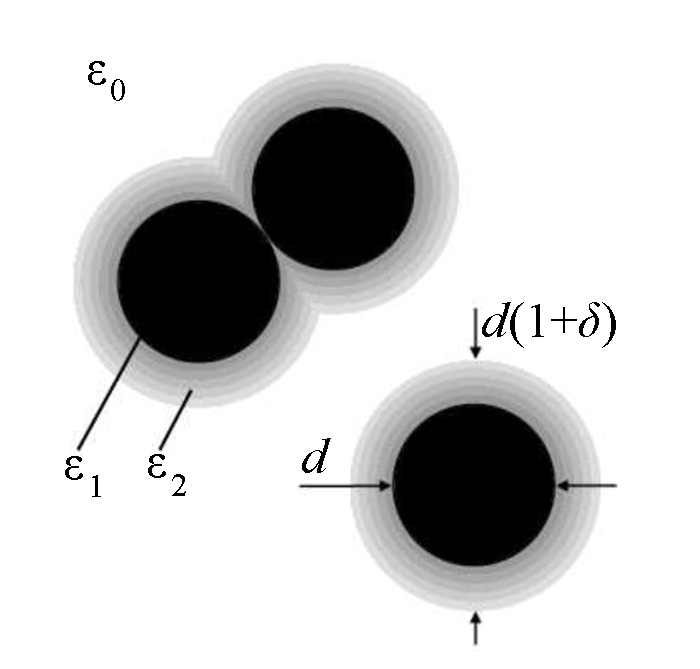
\includegraphics[width=0.3\textwidth]{images/particles-pen.eps}
%   \end{center}
% \vspace{-25pt}
% \end{wrapfigure}
    
% \textbf{Модель тверде ядро--проникна оболонка:}

% {\footnotesize
% \begin{description}
%   \item[білі області] матриця 
%   \item[чорні області] тверді ядра
%   \item[сірі області] проникні оболонки 
% \end{description}
% $$
%     \hat{\varepsilon}({\bf r}) = \left\{ \begin{array}{ll}
%     \hat{\varepsilon}_1, l<R_1 & l = \min\limits_{1 \leq a \leq N} |{\bf r} - {\bf r}_a| \\
%     \hat{\varepsilon}_2, R_1 < l < R_2 & R_1 = d/2 \\
%     \hat{\varepsilon}_0, l > R_2 & R_2 = d(1+\delta)/2
%     \end{array}    
%     \right.
% $$
% \textit{Використання неоднорідних проникних оболонок дозволяє врахувати як міжфазні, 
% так і матричні ефекти.}
% }

% \textbf{Процедура електродинамічної гомогенізації:}\vspace{-5pt}

% {\footnotesize
%     Усі складові системи розглядаються в середовищі, електричні властивості $\hat{\varepsilon}_{\rm f}$ якого знаходяться з фізичних міркувань. 
% }

% \textbf{Теоретична база:}\vspace{-5pt}

% {\footnotesize
%     Розрахунки ефективної квазістатичної комплексної проникності $\hat{\varepsilon}_{\rm eff}$ виконуються в рамках {\bf методу компактних груп}.
% }
% \end{frame}

%%%%%%%%%%%%%%%%%%%%%%%%%%%%%%%%%%%%%%%%%%%%%%%%%%%%%
\begin{frame}{Запропонована модель}

\begin{wrapfigure}{r}{0.3\textwidth}
\vspace{-25pt}
  \begin{center}
    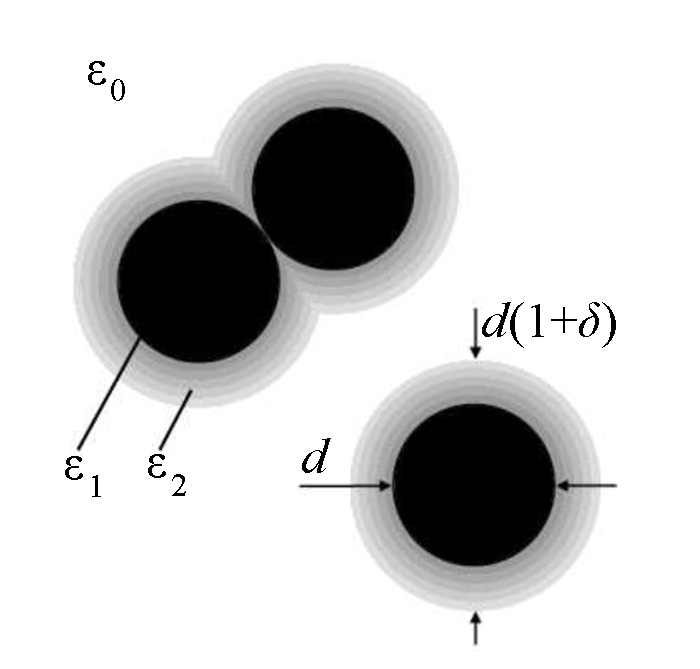
\includegraphics[width=0.3\textwidth]{images/particles-pen.eps}
  \end{center}
\vspace{-25pt}
\end{wrapfigure}
    
Розглядаємо \textbf{макроскопічно однорідні та ізотропні дисперсні системи частинок із морфологією тверде ядро--проникна оболонка:}

\footnotesize
\begin{description}
  \item[білі області] матриця 
  \item[чорні області] тверді ядра
  \item[сірі області] проникні оболонки 
\end{description}
$$
    \hat{\varepsilon}({\bf r}) = \left\{ \begin{array}{ll}
    \hat{\varepsilon}_1, l<R_1 & l = \min\limits_{1 \leq a \leq N} |{\bf r} - {\bf r}_a| \\
    \hat{\varepsilon}_2, R_1 < l < R_2 & R_1 = d/2 \\
    \hat{\varepsilon}_0, l > R_2 & R_2 = d(1+\delta)/2
    \end{array}    
    \right. \vspace{5pt}
$$

Припускаємо, що \textit{використання електрично неоднорідних проникних оболонок, що підкоряються певному правилу домінування, дозволяє ефективно врахувати як міжфазні, так і матричні ефекти.}


Обчислюємо \textit{ефективну квазістатичну проникність} таких систем (частота тестуючого поля $\omega$ достатньо мала, щоб можна було знехтувати діелектричними втратами). 

% Комплексна діелектрична проникність $\hat{\varepsilon}$ у такому наближенні може бути визначена з рівняння неперервності та матеріальних рівнянь у Фур'є-представленні за часом: 
% $$
%     -i\omega \rho + {\rm div}\, {\bf j} = 0;\qquad {\bf D} = \varepsilon{\bf E};\qquad {\bf j} = \sigma {\bf E},
% $$
% звідки отримаємо рівняння для комплексного струму $\bf J$ та $\hat{\varepsilon}$:
% $$
%     {\bf J} = -i\frac{\omega}{4\pi} \hat{\varepsilon} {\bf E};\qquad \hat{\varepsilon} = \varepsilon + i \frac{4\pi\sigma}{\omega},
% $$
% де $\varepsilon$ -- дійсна частина діелектричної проникності; $\sigma$ -- статична провідність; $\rho$, ${\bf j}$ -- щільність вільних зарядів та струму, відповідно; ${\bf D}$, ${\bf E}$ -- вектори індукції та напруженності електричного поля, відповідно.

\end{frame}

%%%%%%%%%%%%%%%%%%%%%%%%%%%%%%%%%%%%%%%%%%%%%%%%%%%%%%%%%%%%%%%%%%%%%%%%%%%%%%%%%%%%%%%%%%%
\section{Теоретична реалізація моделі тверде ядро--проникна оболонка}%%%%%%%%%%%%%%%%%%%%%%
%%%%%%%%%%%%%%%%%%%%%%%%%%%%%%%%%%%%%%%%%%%%%%%%%%%%%%%%%%%%%%%%%%%%%%%%%%%%%%%%%%%%%%%%%%%
\begin{frame}{Основні поняття та співвідношення}

\begin{list}{$\bullet$}{\leftmargin=1em \itemindent=0em}\footnotesize
\item 
Для знаходження квазістатичної діелектричної проникності $\hat{\varepsilon}$ виходимо з рівнянь Максвелла, неперервності та матеріальних рівнянь, записаних у частотному зображенні: 
$$
    {\rm div}\, {\bf D} = 4\pi\rho;\qquad 
    -i\omega \rho + {\rm div}\, {\bf j} = 0
    ;\qquad
    {\bf D} = \varepsilon{\bf E};\qquad 
    {\bf j} = \sigma {\bf E}ю
$$
Звідси дістаємо рівняння для комплексного струму $\bf J$ та $\hat{\varepsilon}$:
$$
    {\bf J} = -i\frac{\omega}{4\pi} \hat{\varepsilon} {\bf E};\qquad \hat{\varepsilon} = \varepsilon + i \frac{4\pi\sigma}{\omega},
$$
де $\varepsilon$ -- дійсна частина діелектричної проникності; $\sigma$ -- статична провідність;  $\rho$, ${\bf j}$ -- густини вільних зарядів та струму; ${\bf D}$, ${\bf E}$ -- вектори індукції та напруженності електричного поля.

\item 
Ефективну квазістатичну $\hat{\varepsilon}_{\rm eff}$ визначаємо із співвідношення
\begin{equation}\label{eq:effcomplex} 
\langle {\bf{J}} ({\bf{r}})\rangle =
-i\frac{\omega}{4\pi}\langle \hat{\varepsilon} ({\bf{r}}) {\bf{E}}
({\bf{r}}) \rangle = -i\frac{\omega}{4\pi} \hat{\varepsilon}_{\rm
eff} \langle {\bf{E}} ({\bf{r}}) \rangle,
\end{equation}
де %${\bf J}({\bf{r}})$ та ${\bf E}({\bf{r}})$ -- локальні значення щільності комплексного струму та напруженості електричного поля; 
кутові дужки позначають статистичне усереднення за положеннями частинок.

\item 
Розрахунки ${\bf J}({\bf{r}})$ та ${\bf E}({\bf{r}})$ виконуються в рамках {\bf методу ``компактних груп неоднорідностей''}.

\end{list}

\end{frame}
%%%%%%%%%%%%%%%%%%%%%%%%%%%%%%%%%%%%%%%%%%%%%%%%%%%%%
\begin{frame}{Фізична інтерпритація методу компактних груп}

\scriptsize{
[М.Я. Сушко, ЖЭТФ {\bf 132} (2007) 478; J. Phys. D: Appl. Phys. {\bf 42} (2009) 155410; Phys. Rev. E {\bf 96} (2017) 062121]
}


\begin{list}{$\bullet$}{\leftmargin=1em \itemindent=0em}\footnotesize

\item 
Припускаємо, що електричний відгук реальної дисперсної системи $\cal{D}$ еквівалентний відгуку допоміжної системи $\cal{S}$, утвореної диспергуванням компонентів $\cal{D}$ в деяку однорідну матрицю $\cal{M}$.

\item

$\cal{S}$ розглядаємо як сукупуність макроскопічних областей (компактних груп), лінійні розміри яких набагато менші ніж довжина хвилі $\lambda$ в $\cal{M}$, але досить великі, щоб формувати властивості всієї $\cal{S}$.

\item
Розподіл комплексної діелектричної проникності в $\cal{S}$ моделюємо у вигляді
$$
    \hat{\varepsilon} ({\bf r}) = \hat{\varepsilon}_{\rm f} + \delta\hat{\varepsilon} ({\bf r}),
$$
де $\hat{\varepsilon}_{\rm f}$ -- проникність $\cal{M}$; $\delta\hat{\varepsilon} ({\bf r})$ -- кусково-неперервна функція, що враховує внесок компактної групи частинок, розташованої в точці $\bf r$.

\end{list}

\end{frame}
%%%%%%%%%%%%%%%%%%%%%%%%%%%%%%%%%%%%%%%%%%%%%%%%%%%%%
\begin{frame}{Знаходження $\langle {\bf J} \rangle$ та $\langle {\bf E} \rangle$}
\footnotesize
%[М.Я. Сушко, ЖЭТФ {\bf 132} (2007) 478; J. %Phys. D: Appl. Phys. {\bf 42} (2009) 155410; %Phys. Rev. E {\bf 96} (2017) 062121]

\begin{list}{$\bullet$}{\leftmargin=1em \itemindent=0em}
\item
Напруженість електричного поля ${\bf E} ({\bf r})$ електромагнітної хвилі в $\cal{S}$ описується рівнянням
\begin{equation} \label{eq:propogating_field}
\Delta {\bf E} + k_0^{2}\hat{\varepsilon}_{\rm f} {\bf E} - {\rm
grad}\, {\rm div} {\bf E} = - k_{0}^{2} \delta
\hat{\varepsilon} {\bf E},
\end{equation}
де $k_0=\omega/c$ -- модуль хвильового вектора ${\bf k}_0$ у вакуумі.

\item
Еквівалентне інтегральне рівняння:
\begin{equation}\label{eq:propogating_field_integral} 
{\rm {\bf E}}({\rm {\bf r}}) = {\rm {\bf E}}_{0} ({\rm
{\bf r}}) - {\int\limits_{V} {d{\rm {\bf {r}'}}\,}} {\rm T}(|{\rm {\bf
r}}-{\rm {\bf {r}'}}|) k_{0}^{2} \delta \hat{\varepsilon} ({\rm
{\bf {r}'}})\,{\rm {\bf E}}({\rm {\bf {r}'}}),
\end{equation}
де ${\bf E}_0 ({\bf r}) = {\bf E}_0 \exp{(i\, {\bf k} \cdot{\bf r})}$ та ${\bf k} = \hat{\varepsilon}_{\rm f}^{1/2} {\bf k}_0$ (з ${\rm Im}{\hat{\varepsilon}_{\rm f}}^{1/2} \geq 0$) -- поле та хвильовий вектор падаючої хвилі в $\cal{M}$;
${\rm T}(r)$ -- тензор Гріна рівняння (\ref{eq:propogating_field}) (пропагатор електричного поля). 

\item
При обчисленні інтеграла (\ref{eq:propogating_field_integral}) підінтегральний пропагатор ${\rm T}(r)$ заміняємо його розкладом [W. Weiglhofer, Am. J. Phys. {\bf 57} (1989) 455] на сингулярну та головну частини:
\begin{eqnarray}\label{eq:propog_representation} 
{\widetilde T}_{\alpha\beta} ({\rm {\bf
r}}) = \frac{1}{3k^{2}} \delta_{\alpha\beta} \delta ({\rm {\bf
r}})\,e^{ikr} + \frac{1}{4\pi k^{2}}
\left(\frac{1}{r^3}-\frac{ik}{r^2}\right)\nonumber\\
\times\left( \delta _{\alpha\beta} - 3e_{\alpha} e_{\beta}
\right)\,e^{ikr} - \frac{1}{4\pi r}\left( {\delta _{\alpha\beta} -
e_{\alpha} e_{\beta}} \right)\,e^{ikr},
\end{eqnarray}
де $\delta({\bf r})$ -- дельта-фукція Дірака; $\delta_{\alpha\beta}$ -- символ Кронекера; $e_\alpha = r_\alpha/|{\bf r}|$.

\end{list}

\end{frame}
%%%%%%%%%%%%%%%%%%%%%%%%%%%%%%%%%%%%%%%%%%%
\begin{frame}{Знаходження $\langle {\bf J} \rangle$ та $\langle {\bf E} \rangle$}
\footnotesize

\begin{list}{$\bullet$}{\leftmargin=1em \itemindent=0em}
\item
У довгохвильовому наближенні 
\begin{equation} \label{representationZerofrequency}
\lim_{\omega \to 0} k_{0}^2 \hat{\varepsilon}_{\rm f} {\widetilde
T}_{\alpha\beta} ({\rm {\bf r}}) = \tau^{(1)}_{\alpha\beta}+
\tau^{(2)}_{\alpha\beta},
\end{equation}
\begin{equation} \label{representationZerofrequencyParts}
\tau^{(1)}_{\alpha\beta}= \frac{1}{3}\,\delta _{\alpha\beta}
\delta ({\rm {\bf r}}), \quad \tau^{(2)}_{\alpha\beta} = \frac{
{\delta _{\alpha\beta} - 3e_{\alpha} e_{\beta}}}{4\pi r^3}.
\end{equation}

\item
Після простих алгебраїчних перетворень отримуємо:
\begin{equation}\label{eq:Eaveraged}
\begin{split}
\langle \mathbf{E} (\mathbf{r}) \rangle = \left\langle \frac{ 3
\hat{\varepsilon}_{\rm f}  }{3 \hat{\varepsilon}_{\rm f}
+ \delta\hat{\varepsilon}({\bf r})} \right\rangle \mathbf{E}_0 
- 3 \int\limits_V {d{\mathbf{r}}'} { {\rm \tau}^{(2)} (| {\bf r}
- {\bf r}' |) \left\langle \frac{\delta \hat{\varepsilon}
({\mathbf{r}}')}{3 \hat{\varepsilon}_{\rm f} + \delta
\hat{\varepsilon}({\bf r})}{\mathbf{E}}({\mathbf{r}}')
\right\rangle },
\end{split}
\end{equation}
\begin{equation}\label{eq:Caveraged}
\begin{split}
\langle \mathbf{J} & (\mathbf{r}) \rangle = -i \frac{\omega}{4\pi}
\, \hat{\varepsilon}_{\rm f}\left[1+ 2\left\langle \frac{
\delta\hat{\varepsilon}({\bf r}) }{3 \hat{\varepsilon}_{\rm f}
+ \delta\hat{\varepsilon}({\bf r})} \right\rangle \right] \mathbf{E}_0 \\
&+i \frac{3}{4\pi}\,  \int\limits_V {d{\mathbf{r}}'} {
{\rm \tau}^{(2)} (| {\bf r} - {\bf r}' |) \left\langle
\frac{\omega\, \hat{\varepsilon}({\bf r}) \,\delta
\hat{\varepsilon} ({\mathbf{r}}')}{3 \hat{\varepsilon}_{\rm f} +
\delta \hat{\varepsilon}({\bf r})}{\mathbf{E}}({\mathbf{r}}')
\right\rangle }.
\end{split}
\end{equation}

\item
Середні під інтегралами залежать лише від $|{\bf r} - {\bf r}'|$, тому після інтегрування за кутами вонидорівнюють нулю внаслідок явного виду кутової частини $\tau_{\alpha\beta}^{(2)}$.

%\item
%З отриманого результату знаходимо вираз для %$\hat{Q}$:
%\begin{equation}
%    \hat{Q}({\bf r}) = - %\frac{\delta\hat{\varepsilon}({\bf r}) }{3 %\hat{\varepsilon}_{\rm f} + %\delta\hat{\varepsilon}({\bf r})}.
%\end{equation}

\end{list}

\end{frame}

%%%%%%%%%%%%%%%%%%%%%%%%%%%%%%%%%%%%%%%%%%%%%%%%%%%%%
\begin{frame}{Знаходження $\hat{\varepsilon}_{\rm f}$}
%\footnotesize
\footnotesize
З граничних умов для нормальних компонент електричного поля на поверхні розділу $\cal{M}$ та $\cal{D}$:
\begin{equation} \label{eq:boundarycondition}
\hat{\varepsilon}_{\rm
f} {\mathbf{E}}_{0n} = \hat{\varepsilon}_{\rm eff}
\left\langle{\mathbf{E}}({\mathbf{r}})\right\rangle_n
\end{equation}
випливає система рівнянь
\begin{equation}
\label{eq:system}
\begin{gathered}
\hat{ \varepsilon}_{\rm f} =\hat{\varepsilon}_{\rm eff}
\left(1+\langle \hat{Q}\rangle\right),\\
\hat{\varepsilon}_{\rm f}\left(1-2\langle \hat{Q}\rangle\right)
=\hat{\varepsilon}_{\rm eff} \left(1+\langle
\hat{Q}\rangle\right),
\end{gathered}
\end{equation}
де $\hat{Q}({\bf r}) = - \cfrac{\delta\hat{\varepsilon}({\bf r}) }{3 \hat{\varepsilon}_{\rm f} + \delta\hat{\varepsilon}({\bf r})}$. За умови, що $\hat{\varepsilon}_{\rm f} \neq 0$, дістаємо:
\begin{equation} \label{eq:ef} 
\hat{ \varepsilon}_{\rm f} = \hat{ \varepsilon}_{\rm eff},
\end{equation}
\begin{equation} \label{eq:equation}
\langle \hat{Q}({\mathbf{r}})\rangle  = 0,
\end{equation}
що дає рівняння для знаходження $\hat{\varepsilon}_{\rm eff}$:
\begin{equation} \label{eq:equation}
\boxed{
\left\langle \frac{\delta\hat{\varepsilon}({\bf r}) }{3 \hat{\varepsilon}_{\rm eff} + \delta\hat{\varepsilon}({\bf r})} \right\rangle = 0.
}
\end{equation}

\end{frame}

%%%%%%%%%%%%%%%%%%%%%%%%%%%%%%%%%%%%%%%%%%%%%%%%%%%%%
\begin{frame}{Моделювання $\delta\hat{\varepsilon}({\bf r})$}
\footnotesize

\begin{wrapfigure}{r}{0.45\textwidth}
\vspace{-25pt}
  \begin{center}
    \includegraphics[width=0.45\textwidth]{images/Fig1_Microstructure_new5.eps}
  \end{center}
\vspace{-15pt}
\end{wrapfigure}

Для випадку $\hat{\varepsilon}_2 = const$:
\begin{equation}
\begin{split}
    \delta\hat{\varepsilon}({\bf r}) = [1 - \Pi_2({\bf r})]\Delta\hat{\varepsilon}_0 + \Pi_1({\bf r}) \Delta\hat{\varepsilon}_1 \\
    + [\Pi_2({\bf r}) - \Pi_1({\bf r})]\Delta\hat{\varepsilon}_2,
\end{split}
\end{equation}
де
$$
    \Delta\hat{\varepsilon}_q = \hat{\varepsilon}_{q} - \hat{\varepsilon}_{\rm f}, \quad q=0,1,2,
$$ та введено такі характеристичні функції: 
$$
    \Pi_1 ({\bf r}) = \sum\limits_{a=1}^N \chi_a^{(1)} ({\bf r})
$$
-- області, зайнятої твердими ядрами ($\chi_a^{(1)}({\bf r})$ -- характеристична функція ядра $a$-ої частинки);
$$
    \Pi_2 ({\bf r}) = 1 - \prod\limits_{a=1}^N [1 - \chi_a^{(2)} ({\bf r})];
$$
-- області, зайнятої твердими ядрами разом з проникними оболонками;
($\chi_a^{(2)}({\bf r})$ -- характеристична функція $a$-ої частинки (її ядра та оболонки)).\vspace{5pt}\\

Для сферичних частинок $\chi_a^{(q)}({\bf r}) = \theta(R_q - |{\bf r} - {\bf r}_a|)$ -- ступінчаста функція Хевісайда.

\end{frame}


%%%%%%%%%%%%%%%%%%%%%%%%%%%%%%%%%%%%%%%%%%%%%%%%%%%%%
\begin{frame}{Результати для випадку однорідних оболонок}
\footnotesize

\begin{list}{$\bullet$}{\leftmargin=1em \itemindent=0em}
\item
Рівняння для $\hat{\varepsilon}_{\rm eff}$:
\begin{equation}\label{eq:uniformshell}
\boxed{
\left[1-\phi(c, \delta)\right]\frac{\hat{\varepsilon}_0
-\hat{\varepsilon}_{\rm eff}}{2\hat{\varepsilon}_{\rm
eff}+\hat{\varepsilon}_0} + c\,\frac{\hat{\varepsilon}_1
-\hat{\varepsilon}_{\rm eff}}{2\hat{\varepsilon}_{\rm
eff}+\hat{\varepsilon}_1}
+\left[\phi(c, \delta)-c\right]\frac{\hat{\varepsilon}_2
-\hat{\varepsilon}_{\rm eff}}{2\hat{\varepsilon}_{\rm
eff}+\hat{\varepsilon}_2}=0, 
}
\end{equation}
де $c = \langle \Pi_1 \rangle$ -- об'ємна концентрація ядер; $\phi = \langle \Pi_2 \rangle$ -- об'ємна концентрація ядер з оболонками. 

\item
За умови, що  $|\sigma_{\rm eff}-\sigma_{ q}|  \gg  
\left(2\varepsilon_{\rm eff} +\varepsilon_q \right) \omega/4\pi$ для всіх $q=0,1,2$,  рівняння для квазістатичної провідності має вигляд:
\begin{equation}\label{eq:conductivity}
\boxed{
\left[1-\phi(c, \delta)\right]\frac{\sigma_0 -\sigma_{\rm
eff}}{2\sigma_{\rm eff}+\sigma_0} + c\,\frac{\sigma_1 -\sigma_{\rm
eff}}{2\sigma_{\rm eff}+\sigma_1} 
+\left[\phi(c, \delta)-c\right]\frac{\sigma_2 -\sigma_{\rm
eff}}{2\sigma_{\rm eff}+\sigma_2}=0. 
}
\end{equation}
У статичному випадку воно є \textbf{строгим}.

\item
Для сферичних частинок $\phi$ знайдено статистичними методами в рамках суперпозиційного підходу Кірквуда, строгого на рівні третього вірального коефіцієнта  [P.~Rikvold, G.~Stell, J. Coll. and Int. Sci. {\bf 108} (1985) 158],
\begin{equation}\label{effectiveconcentration}
\begin{split}
\phi(c,\delta)= 1-
(1 - c)\,\exp\left[{-\frac{((1+\delta)^3 -
1)c}{1-c}}\right] \\
 \times  \exp\left\{
- \frac{3(1 + \delta)^3
c^2}{2(1 - c)^3} \left[2 - \frac{3}{1+\delta} +
\frac{1}{(1+\delta)^3} \right. \right. \\
- \left. \left. \left( \frac{3}{1+\delta} -
\frac{6}{(1+\delta)^2} + \frac{3}{(1+\delta)^3}\right) c
\right]\right\}. 
\end{split}
\end{equation}

\end{list}

\end{frame}

%%%%%%%%%%%%%%%%%%%%%%%%%%%%%%%%%%%%%%%%%%%%%%%%%%%%%
\begin{frame}{Узагальнення на електрично неоднорідні оболонки}
\footnotesize

\begin{wrapfigure}{r}{0.35\textwidth}
\vspace{-20pt}
  \begin{center}
    \includegraphics[width=0.35\textwidth]{images/2shell.png}
  \end{center}
\vspace{-25pt}
\end{wrapfigure}

\begin{equation*} 
\hat{\varepsilon}({\bf r})=\begin{cases}
\hat{\varepsilon}_1 & {\text{if} } \quad \,\,l<R_1, \qquad l=\min\limits_{1 \leq a \leq N} |{\bf r} - {\bf r}_a| \\
\hat{\varepsilon}_{2,1} & {\text{if} }\quad  R_1<l<R_{2,1},\\
{\hat{\varepsilon}_{2,m}} & \text{if} \quad { R_{2,m-1}<l<R_{2,m}, \,2 \leq m \leq M},\\
\hat{\varepsilon}_0 & {\text{if} }\quad \,\, l>R_{2,M}.
\end{cases} \label{distr1}
\end{equation*}
Відповідно
\begin{equation}
\begin{split}
\delta\hat{\varepsilon} ({\bf r}) = \left[1- \Pi_{2,M}({\bf
r})\right] \Delta\hat{\varepsilon}_0
+ \Pi_1({\bf r}) \Delta\hat{\varepsilon}_1
+  \left[\Pi_{2,1}({\bf r})
-\Pi_1({\bf r})  \right] \Delta\hat{\varepsilon}_{2,1} \\
+ {\sum\limits_{m=2}^M  \left[ \Pi_{2,m}({\bf r}) -
\Pi_{2,m-1}({\bf r}) \right] \Delta\hat{\varepsilon}_{2,m}},
\end{split}
\end{equation}
Після відповідних обчислень та переходу до границі $M \to \infty$ ($\delta_M = const$)  отримуємо:
\begin{equation}\label{eq:nonuniformshell}
\boxed{
\left[1-\phi(c, \delta_M)\right]\frac{\hat{\varepsilon}_0
-\hat{\varepsilon}_{\rm eff}}{2\hat{\varepsilon} _{\rm
eff}+\hat{\varepsilon}_0}+ c\,\frac{\hat{\varepsilon}_1
-\hat{\varepsilon}_{\rm eff}}{2\hat{\varepsilon}_{\rm
eff}+\hat{\varepsilon}_1}
+\int\limits_0^{\delta_M}\frac{\partial \phi(c,u)}{\partial
u}\frac{\hat{\varepsilon}_2 (u) -\hat{\varepsilon}_{\rm
eff}}{2\hat{\varepsilon}_{\rm eff}+\hat{\varepsilon}_2 (u)}\,du
=0
}
\end{equation}
\begin{equation}\label{eq:nonuniformconductivity}
\boxed{
\left[1-\phi(c, \delta_M)\right]\frac{\sigma_0 -\sigma_{\rm
eff}}{2\sigma _{\rm eff}+\sigma_0}+ c\,\frac{\sigma_1 -\sigma_{\rm
eff}}{2\sigma_{\rm eff}+\sigma_1} 
+\int\limits_0^{\delta_M}\frac{\partial \phi(c,u)}{\partial
u}\frac{\sigma_2 (u) -\sigma_{\rm eff}}{2\sigma_{\rm eff}+\sigma_2
(u)}\,du =0.
}
\end{equation}

\end{frame}

%%%%%%%%%%%%%%%%%%%%%%%%%%%%%%%%%%%%%%%%%%%%%%%%%%%%%%%%%%%%%%%%%%%%%%%%%%%%%%%%%%%%%%%%%%%
\section{Тестування моделі на результатах числових симуляцій}%%%%%%%%%%%%%%%%%%%%%%%%%%%%%%%
%%%%%%%%%%%%%%%%%%%%%%%%%%%%%%%%%%%%%%%%%%%%%%%%%%%%%%%%%%%%%%%%%%%%%%%%%%%%%%%%%%%%%%%%%%

\begin{frame}{Тестування теорії на результатах симуляцій RRN}

{\footnotesize
Симуляції: [M. Siekierski et al., Electrochimica Acta {\bf 50} (2005) 3796; 
J. New Mat. Electrochem. Systems {\bf 9} (2006) 375;
J. Pow. Sour. {\bf 173} (2007) 748]
}

\begin{figure}[tb]
    \centering
    \includegraphics[width=0.7\textwidth]{images/RRN.png}
    \caption{Схематичне зображення алгоритму Random Resistor Network (RRN): a) модельна система типу ядро-оболонка; b) її апроксимація системою кубів; c) отримана тривимірна кубічна гратка резисторів.\\ {\footnotesize (Рис. взято з [M. Siekierski, K. Nadara, J. Pow. Sour. {\bf 173} (2007) 748])}}
\end{figure}
\vspace{-10pt}
Концентрації ядер в системах a) та b) рівні: $c=c'$, тоді відповідні відносні товщини будуть зв'язані співвідношенням:
$$
    \delta = K\delta'
$$
$$
    k \leq K \leq 1, \qquad k=(\pi/6)^{1/3}
$$

\end{frame}

%%%%%%%%%%%%%%%%%%%%%%%%%%%%%%%%%%%%%%%%%%%%%%%%%%%%%
%{\setbeamertemplate{frame footer}{Симуляції: [M. Siekierski, K. Nadara, J. Pow. Sour. {\bf 173} (2007) 748]}
\begin{frame}{Тестування зв'язку геометричних параметрів моделей a) та b)}

{ Об'ємні концентрації оболонок товщиною $t=5$~мкм як функції $c$.}
\vspace{-5pt}

\scriptsize{Симуляції: [M. Siekierski, K. Nadara, J. Pow. Sour. {\bf 173} (2007) 748]}
\vspace{-5pt}

\footnotesize
\begin{columns}[T,onlytextwidth]
    \column{0.5\textwidth}
      \begin{figure}
        \centering
        \qquad Діаметр ядра $d=7$~мкм
        \includegraphics[width=0.99\textwidth]{images/Fig2_SiekierskiShell_107.eps}
      \end{figure}

    \column{0.5\textwidth}
      \begin{figure}
        \centering
        \qquad Діаметри ядер $d=3,5,9$~мкм
        \includegraphics[width=0.99\textwidth]{images/Fig3_SiekierskiShell_103-9.eps}
      \end{figure}
\end{columns}

\begin{columns}[T,onlytextwidth]
    \column{0.6\textwidth}
      \vspace{10pt}
      Середньоквадратична похибка:
      $$
        \Delta_a = \sqrt{\frac{1}{N}\sum\limits_{i=1}^N (a_i - \tilde{a}_i)^2}
      $$

    \column{0.4\textwidth}
      \begin{table}
        %\caption{Largest cities in the world (source: Wikipedia)}
        \begin{tabular}{ll}
          \toprule
          Експеримент & $\Delta_{\phi-c}$\\
          \midrule
          $\circ$ $t=0$~мкм & 0.0024\\
          $\blacklozenge$ $d=3$~мкм & 0.0053\\
          $\blacksquare$ $d=5$~мкм & 0.011\\
          $\blacktriangle$ $d=7$~мкм & 0.014\\
          $\bullet$ $d=9$~мкм & 0.0097\\
          \bottomrule
        \end{tabular}
      \end{table}
\end{columns}

\end{frame}
%}
%%%%%%%%%%%%%%%%%%%%%%%%%%%%%%%%%%%%%%%%%%%%%%%%%%%%%
%{\setbeamertemplate{frame footer}{Симуляції: [M. Siekierski, K. Nadara, Electrochimica Acta {\bf 50} (2005) 3796]}
\begin{frame}{Порівняння з числовими даними з провідності}
Концентраційна залежність ефективної провідності при фіксованих $t$ (зліва) та $d$ (справа) з різними значеннями $K$.
\vspace{-5pt}

\scriptsize{Симуляції: [M. Siekierski, K. Nadara, Electrochimica Acta {\bf 50} (2005) 3796]}

\footnotesize
\begin{columns}[T,onlytextwidth]
    \column{0.5\textwidth}
      \begin{figure}
        \centering
        { \qquad Товщина оболонки $t=5$~мкм}
        \includegraphics[width=0.99\textwidth]{images/Fig6_Siekierski_HomogeneousLayers_t_fixed.eps}
      \end{figure}

    \column{0.5\textwidth}
      \begin{figure}
        \centering
        { \qquad Діаметр ядра $d=5$~мкм}
        \includegraphics[width=0.99\textwidth]{images/Fig7_Siekierski_HomogeneousLayers_d_fixed.eps}
      \end{figure}
\end{columns}

\begin{columns}[T,onlytextwidth]
    \column{0.6\textwidth}
      \vspace{10pt}
      Середньоквадратична відносна похибка:
      $$
        \bar{\Delta}_a = \sqrt{\frac{1}{N}\sum\limits_{i=1}^N \left( \frac{a_i - \tilde{a}_i}{a_i} \right)^2}
      $$

    \column{0.4\textwidth}
      \begin{table}
        %\caption{Largest cities in the world (source: Wikipedia)}
        \begin{tabular}{ll}
          \toprule
          Експеримент & $\max \bar{\Delta}_{\sigma_{\rm eff}/\sigma_0}$\\
          \midrule
          $t=5$~мкм & 0.40 | 0.048\\
          $d=5$~мкм & 0.35 | 0.019\\
          \bottomrule
        \end{tabular}
      \end{table}
\end{columns}
\end{frame}
%}

%%%%%%%%%%%%%%%%%%%%%%%%%%%%%%%%%%%%%%%%%%%%%%%%%%%%%
%{\setbeamertemplate{frame footer}{Симуляції: [M. Siekierski et al., J. New Mat. Electrochem. Systems {\bf 9} (2006) 375]}
\begin{frame}{Тестування моделі для випадку неоднорідних оболонок}
Концентраційна залежність ефективної провідності з різними значеннями $K$ для гаусового профілю оболонок.
\vspace{-5pt}

\scriptsize{Симуляції: [M. Siekierski et al., J. New Mat. Electrochem. Systems {\bf 9} (2006) 375]}

\footnotesize
\begin{columns}[T,onlytextwidth]
    \column{0.5\textwidth}
      \begin{figure}
        \centering
        { \qquad Товщина оболонки $t=5$~мкм}
        \includegraphics[width=0.99\textwidth]{images/Fig10_Siekierski_t_fixed.eps}
        $\max \bar{\Delta}_{\sigma_{\rm eff}/\sigma_0} \approx 0.41\,|\,0.048$\\
      \end{figure}

    \column{0.5\textwidth}
      \begin{figure}
        \centering
        { \qquad Діаметр ядра $d=5$~мкм}
        \includegraphics[width=0.99\textwidth]{images/Fig11_Siekierski_d_fixed.eps}
        $\max \bar{\Delta}_{\sigma_{\rm eff}/\sigma_0} \approx 0.28\,|\,0.28$
      \end{figure}
\end{columns}

\end{frame}
%}

%%%%%%%%%%%%%%%%%%%%%%%%%%%%%%%%%%%%%%%%%%%%%%%%%%%%%%%%%%%%%%%%%%%%%%%%%%%%%%%%%%%%%%%%%%%
\section{Застосування до аналізу композитних електролітів}%%%%%%%%%%%%%%%%%%%%%%%%%%%%%%%
%%%%%%%%%%%%%%%%%%%%%%%%%%%%%%%%%%%%%%%%%%%%%%%%%%%%%%%%%%%%%%%%%%%%%%%%%%%%%%%%%%%%%%%%%%
%\subsection{Тестування моделі на числових результатах симуляцій}

%%%%%%%%%%%%%%%%%%%%%%%%%%%%%%%%%%%%%%%%%%%%%%%%%%%%%
%\subsection{Порівняння з експериментальними даними}

%{\setbeamertemplate{frame footer}{Експеримент: [C.C. Liang, J. Electrochem. Soc., {\bf 120} (1973) 1289]}
\begin{frame}{Порівняння теорії з експериментальними даними -- 1}
Концентраційна залежність провідності систем $\rm LiI/Al_2O_3$.
\vspace{-5pt}

\scriptsize{Експеримент: [C.C. Liang, J. Electrochem. Soc., {\bf 120} (1973) 1289]}
\vspace{-10pt}

\footnotesize
\begin{columns}[T,onlytextwidth]
    \column{0.5\textwidth}
      \begin{figure}
        \centering
        %{ \qquad Діаметр ядра $d=7$~мкм}
        \includegraphics[width=0.99\textwidth]{images/Fig12_Liang_LiI-Al2O3-Processing.eps}
        $\sigma_0 \approx 2.5 \times 10^{-7}$~С/см\\
        подвійні оболонки - $\bar{\Delta}_{\sigma_{\rm eff}/\sigma_0} \approx 0.143$\\
        неперервний профіль - $\bar{\Delta}_{\sigma_{\rm eff}/\sigma_0} \approx 0.163$
      \end{figure}

    \column{0.5\textwidth}
      \begin{figure}
        \centering
        { \qquad Профіль провідності}
        \includegraphics[width=0.95\textwidth]{images/Fig13_Liang_LiI-Al2O3-Profile.eps}\\
        \includegraphics[width=0.75\textwidth]{images/Fig14_Liang_LiI-Al2O3-Matrix_2.eps}
      \end{figure}
      
\end{columns}

\end{frame}
%}
%%%%%%%%%%%%%%%%%%%%%%%%%%%%%%%%%%%%%%%%%%%%%%%%%%%%%
%{\setbeamertemplate{frame footer}{Експеримент: [W. Wieczorek, M. Siekierski, J. Appl. Phys. {\bf 76} (1994) 2220;\par J. Przyluski, M. Siekierski, W. Wieczorek, Electrichimica A. {\bf 40} (1995) 2101]}
\begin{frame}{Порівняння теорії з експериментальними даними -- 2}
Ефективна провідність полімерних композитних електролітів $\rm (PEO)NaI-NASICON$ та $\rm (PEO)NaI-\theta Al_2O_3$.
\vspace{-5pt}

\scriptsize{Експеримент: [W. Wieczorek, M. Siekierski, J. Appl. Phys. {\bf 76} (1994) 2220; J. Przyluski, M. Siekierski, W. Wieczorek, Electrichimica A. {\bf 40} (1995) 2101]}
\vspace{-5pt}

\footnotesize
\begin{columns}[T,onlytextwidth]
    \column{0.5\textwidth}
      \begin{figure}
        \centering
        %{ \qquad Діаметр ядра $d=7$~мкм}
        \includegraphics[width=0.99\textwidth]{images/Fig2_PEO-NaI_NASICON_PEO-NaI-theta-Al2O3.eps}
        1d -- $\bar{\Delta}_{\sigma_{\rm eff}/\sigma_0} \approx 0.17$\\
        2d -- $\bar{\Delta}_{\sigma_{\rm eff}/\sigma_0} \approx 0.37$
      \end{figure}

    \column{0.5\textwidth}
      \begin{figure}
        %\centering
        %{ \qquad Одночастинковий профіль провідності}
          \begin{center}
            \begin{overpic}[width=0.99\textwidth]{images/Fig2_PEO-NaI_NASICON_Profile.eps}
                 \put(45,50){\scriptsize $\sigma_0 = 9.86 \times 10^{-9}$~С/см}
            \end{overpic}
            \begin{overpic}[width=0.99\textwidth]{images/Fig2_PEO-NaI-theta-Al2O3_Profile.eps}
                 \put(45,15){\scriptsize $\sigma_0 = 1.54 \times 10^{-8}$~С/см}
            \end{overpic}
          \end{center}
        %\includegraphics[width=0.99\textwidth]{images/Fig2_PEO-NaI_NASICON_Profile.eps}
        %\includegraphics[width=0.99\textwidth]{images/Fig2_PEO-NaI-theta-Al2O3_Profile.eps}
      \end{figure}
      
\end{columns}

\end{frame}
%}
%%%%%%%%%%%%%%%%%%%%%%%%%%%%%%%%%%%%%%%%%%%%%%%%%%%%%
%{\setbeamertemplate{frame footer}{Експеримент: [W. Wieczorek, M. Siekierski, J. Appl. Phys. {\bf 76} (1994) 2220;\par W. Wieczorek et al, J. Phys. Chem. {\bf 98} (1994) 6840]}
\begin{frame}{Порівняння теорії з експериментальними даними -- 3}
Ефективна провідність полімерних композитних електролітів $\rm (PEO)LiClO_4-PAAM$ та $\rm (OMPEO)LiClO_4-PAAM$.
\vspace{-5pt}

\scriptsize{Експеримент: [W. Wieczorek, M. Siekierski, J. Appl. Phys. {\bf 76} (1994) 2220; W. Wieczorek et al, J. Phys. Chem. {\bf 98} (1994) 6840]}
\vspace{-5pt}

\footnotesize
\begin{columns}[T,onlytextwidth]
    \column{0.5\textwidth}
      \begin{figure}
        \centering
        %{ \qquad Діаметр ядра $d=7$~мкм}
        \includegraphics[width=0.99\textwidth]{images/Fig3_PEO-PAAM_LiClO4_OMPEO-PAAM_LiClO4.eps}
        3c -- $\bar{\Delta}_{\sigma_{\rm eff}/\sigma_0} \approx 0.29$\\
        4c -- $\bar{\Delta}_{\sigma_{\rm eff}/\sigma_0} \approx 0.33$
      \end{figure}

    \column{0.5\textwidth}
      \begin{figure}
        %\centering
        %{ \qquad Одночастинковий профіль провідності}
        %\includegraphics[width=0.99\textwidth]{images/Fig3_PEO-PAAM_LiClO4_Profile.eps}
        %$\sigma_0 = 13.1$~мкС/см
          \begin{center}
            \begin{overpic}[width=0.99\textwidth]{images/Fig3_PEO-PAAM_LiClO4_Profile.eps}
                 \put(45,15){\scriptsize $\sigma_0 = 6.21 \times 10^{-7}$~С/см}
            \end{overpic}
            \begin{overpic}[width=0.99\textwidth]{images/Fig3_OMPEO-PAAM_LiClO4_Profile.eps}
                 \put(45,15){\scriptsize $\sigma_0 = 1.61 \times 10^{-5}$~С/см}
            \end{overpic}
          \end{center}
        %\includegraphics[width=0.99\textwidth]{images/Fig3_OMPEO-PAAM_LiClO4_Profile.eps}
        %$\sigma_0 = 13.1$~мкС/см
      \end{figure}
      
\end{columns}

\end{frame}
%}
%%%%%%%%%%%%%%%%%%%%%%%%%%%%%%%%%%%%%%%%%%%%%%%%%%%%%
{\setbeamertemplate{frame footer}{Експеримент: [W. Wieczorek, M. Siekierski, J. Appl. Phys. {\bf 76} (1994) 2220;\par W. Wieczorek et al, J. Phys. Chem. {\bf 98} (1994) 6840]}
\begin{frame}{Порівняння з іншими теоріями}
Ефективна провідність полімерних композитних електролітів $\rm (PEO)LiClO_4-PAAM$ та $\rm (OMPEO)LiClO_4-PAAM$

\footnotesize
неперервні лінії -- наш підхід; 
штрихован лінії -- підхід Нана--Вєчорика


      \begin{figure}
        \centering
        %{ \qquad Діаметр ядра $d=7$~мкм}
        \includegraphics[width=0.6\textwidth]{images/Fig5_Comparison.eps}
      \end{figure}

\end{frame}
}
%%%%%%%%%%%%%%%%%%%%%%%%%%%%%%%%%%%%%%%%%%%%%%%%%%%%%
%{\setbeamertemplate{frame footer}{Експеримент: [W. Wieczorek et al, J. Phys. Chem. {\bf 98} (1994) 6840]}
\begin{frame}{Розширення моделі: температурна залежність провідності}
Ефективна провідність полімерних композитних електролітів $\rm (OMPEO)LiClO_4-PAAM$.
\vspace{-5pt}

\scriptsize{Експеримент: [W. Wieczorek et al, J. Phys. Chem. {\bf 98} (1994) 6840]}
\vspace{-5pt}
\footnotesize
\begin{columns}[T,onlytextwidth]
    \column{0.5\textwidth}
      \begin{figure}
        %{ \qquad Діаметр ядра $d=7$~мкм}
          \begin{center}
            \begin{overpic}[width=0.99\textwidth]{images/Fig6_Isochores.eps}
                 \put(45,20){$t = 0^{o} C$}
                 \put(45,57){$t = 25^{o} C$}
                 \put(45,78){$t = 100^{o} C$}
            \end{overpic}
          \end{center}
        %\includegraphics[width=0.99\textwidth]{images/Fig6_Isochores.eps}
        $\max \bar{\Delta}_{\sigma_{\rm eff}} \approx 0.41$
      \end{figure}

    \column{0.5\textwidth}
      \begin{figure}
        \centering
        %{ \qquad Одночастинковий профіль провідності}
        %\includegraphics[width=0.99\textwidth]{images/Fig8_TemperatureDependence_1.eps}
          \begin{center}
            \begin{overpic}[width=0.99\textwidth]{images/Fig8_TemperatureDependence_1.eps}
                 \put(33,30){$\bigtriangledown:\, c = 0.05$}
                 \put(34,25){$\square:\, c = 0.25$}
                 \put(34,20){$\blacktriangle:\, c = 0.40$}
                 \put(35,15){$\bullet:\, c = 0.50$}
            \end{overpic}
          \end{center}
        $\max \bar{\Delta}_{\sigma_{\rm eff}} \approx 0.35$
      \end{figure}
      
\end{columns}

Емпіричний закон Vogel-Tamman-Fulcher (VTF) для полімерів:
$$
    \sigma = \frac{A}{\sqrt{T}}\exp{\left( -\frac{B}{T-T_0} \right)}.
$$

\end{frame}
%}

%%%%%%%%%%%%%%%%%%%%%%%%%%%%%%%%%%%%%%%%%%%%%%%%%%%%%%%%%%%%%%%%%%%%%%%%%%%%%%%%%%%%%%%%%%%
\section{Аналіз ефекту перколяції в рамках моделі}%%%%%%%%%%%%%%%%%%%%%%%%%%%%%%%
%%%%%%%%%%%%%%%%%%%%%%%%%%%%%%%%%%%%%%%%%%%%%%%%%%%%%%%%%%%%%%%%%%%%%%%%%%%%%%%%%%%%%%%%%%
\subsection{Поріг та критичні індекси перколяції}

\begin{frame}{Аналіз моделі у випадку непровідної матриці}
\footnotesize

Для непровідної матриці ($\sigma_0 \to 0$) та електрично однорідної оболонки отримаємо:
\begin{equation*}
    x = \frac{3}{4} \left\{ \left( c - \frac{1}{3} \right) + \left(\phi - c - \frac{1}{3} \right)x_2 \pm \sqrt{\frac{4}{3}\left( \phi - \frac{1}{3} \right) x_2 + \left[ \left( c - \frac{1}{3} \right) + \left( \phi - c - \frac{1}{3} \right)x_2 \right]^2 } \right\},
\end{equation*}
$$
     x = \sigma_{\rm eff}/\sigma_1, \qquad x_2 = \sigma_2/\sigma_1
$$

\begin{columns}[T,onlytextwidth]
    \column{0.5\textwidth}
      \begin{figure}
        \centering
        Поріг перколяції $c_c$: $\phi(c_c, \delta) = 1/3$
        \includegraphics[width=0.99\textwidth]{images/cc-delta.png}
        Залежність $c_c$ від відносної товщини $\delta$
для проникних (неперервна) та твердих (штрихована) оболонок.
      \end{figure}

    \column{0.5\textwidth}
        \vspace{8pt}
        Перколяційні критичні індекси провідності:
        $$x \sim (c-c_c)^t, \quad (c \to c_c+0)$$
        $$x \sim (c_c-c)^{-s}, \quad (c \to c_c-0)$$
        Наша модель:
        $$
            t=s=1
        $$
        Теорія:
        $$
            t \approx 1.3 \div 2.14
        $$
        $$
            s \approx 0.75
        $$
    %   \begin{figure}
    %     \centering
    %     Положення максимуму провідності $c_m$: $\partial \phi/\partial c|_{c_m} = 1$ \underline{(у випадку $\sigma_2 \gg \sigma_1$)}
    %     \includegraphics[width=0.85\textwidth]{images/Fig8_Siekierski_MaximumLocation.eps}
    %     Точки -- дані симуляцій [M. Siekierski et al., Electrochimica Acta {\bf 50} (2005) 3796]
    %   \end{figure}
      
\end{columns}

\end{frame}
%%%%%%%%%%%%%%%%%%%%%%%%%%%%%%%%%%%%%%%%%%%%%%%%%%%%%
\begin{frame}{Ефективні критичні індекси перколяції}
\footnotesize

%\vspace{-15pt}
\begin{columns}[T,onlytextwidth]
    \column{0.5\textwidth}
      \begin{figure}
        \centering
        Експеримент: $t\approx 1.5 \div 2.0$ та вище
        %$$x \sim (c-c_c)^t, \quad (c \to c_c+0)$$
        $$t_{\rm eff} = ln \frac{\sigma(c_2)}{\sigma(c_1)} / ln \frac{c_2-c_c}{c_1 - c_c}, \quad (c>c_c)$$
        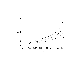
\includegraphics[width=0.99\textwidth]{images/teff.eps}
      \end{figure}
        Залежність ефективного індексу $t_{\rm eff}$ від $c_2$ при фіксованих $c_1$, $\delta=0.1$ ($c_c \approx 0.251$) та $x_2 = 5\times 10^{-5}$. Звурху вниз: $c_1 = 0.26, 0.27, 0.28$.\\
        %Теорія перколяцій: $t \approx 1.3 \div 2.14$\\
        %Експеримент: $t\approx 1.5 \div 2.0$ та вище

    \column{0.5\textwidth}
      \begin{figure}
        \centering
        Експеримент: $s\approx 0.7 \div 1.0$
        %$$x \sim (c_c-c)^{-s}, \quad (c \to c_c-0)$$
        $$s_{\rm eff} = - ln \frac{\sigma(c_2)}{\sigma(c_1)} / ln \frac{c_c-c_2}{c_c - c_1}, \quad (c<c_c)$$
        \includegraphics[width=0.99\textwidth]{images/seff.eps}
      \end{figure}
      \hfill
      \begin{minipage}[t]{0.9\textwidth}
        Залежність ефективного індексу $s_{\rm eff}$ від $x_0 = \sigma_0/\sigma_1$ при  $\delta=0.1$ ($c_c \approx 0.251$), $x_2 = 5\times 10^{-5}$, $c_1 = 0.24$ та $c_2 = 0.25$.\\
        %Теорія перколяцій: $s \approx 0.75$\\
        %Експеримент: $s\approx 0.7 \div 1.0$
      \end{minipage}
\end{columns}

\end{frame}
%%%%%%%%%%%%%%%%%%%%%%%%%%%%%%%%%%%%%%%%%%%%%%%%%%%%%
\begin{frame}{Ефект подвійної перколяції}
\footnotesize

\vspace{-10pt}
\begin{columns}[T,onlytextwidth]
    \column{0.5\textwidth}
      \begin{figure}
        \centering
        \includegraphics[width=0.99\textwidth]{images/Permit5.eps}
      \end{figure}
        \vspace{-10pt}
        Залежність відносної провідності 
 ($x = \sigma_{\rm eff}/\sigma_1$) системи від 
концентрації твердих ядер $c$ 
при різних значеннях відносної 
товщини $\delta$ міжфазної границі.\\            
Штрихована лінія -- перколяція ($\delta=0$)\\
Неперерва лінія -- ``подвійна'‘ перколяція
($\delta=0.05$, $x_2 = 5 \times 10^{-5}$, $x_0 = 1 \times 10^{-10}$)                             

    \column{0.5\textwidth}
      \begin{figure}
        \centering
        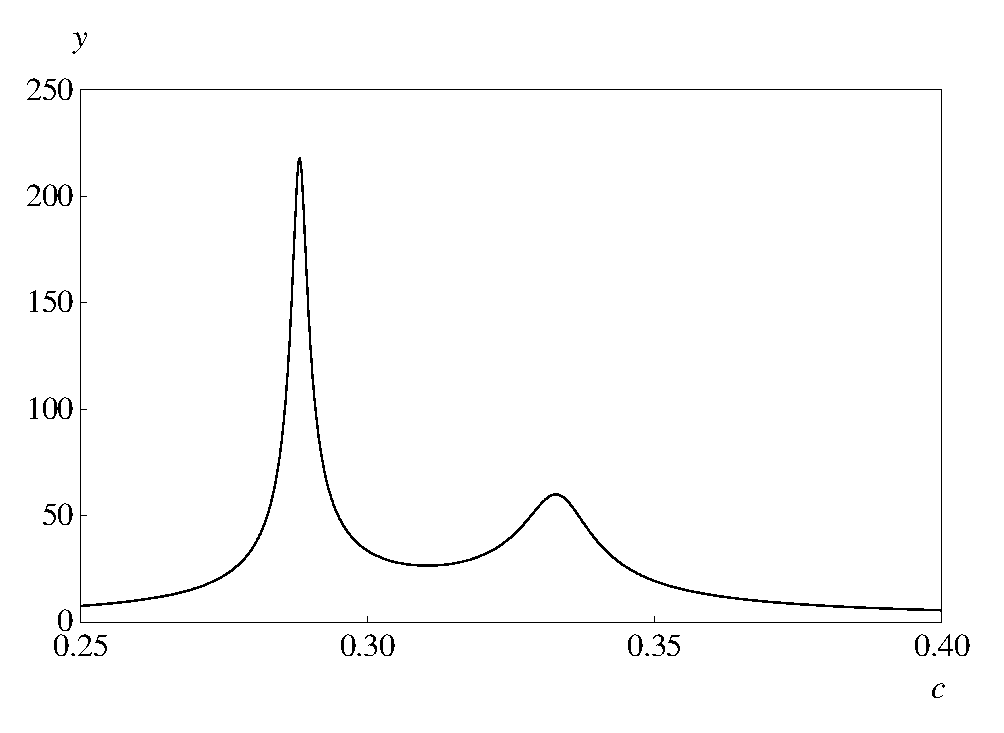
\includegraphics[width=0.99\textwidth]{images/Permit1.eps}
      \end{figure}
        \vspace{-10pt}\hfill
      \begin{minipage}[t]{0.9\textwidth}
        Залежність дійсної частини ефективної проникності ($y = \varepsilon_{\rm eff}/\varepsilon_1$) від концентрації ядер $c$. Параметри: $x_2 = 5 \times 10^{-4}$, $y_1 = 1.5$, $y_2=1$, $\delta=0.05$.
        
        \vspace{20pt}
Експериментальне підтверждення для ЖК систем: [S. Tomylko et al., Phys. Rev. E {\bf 92(1)} (2015) 012502]
      \end{minipage}
\end{columns}
\end{frame}


%%%%%%%%%%%%%%%%%%%%%%%%%%%%%%%%%%%%%%%%%%%%%%%%%%%%%
\subsection{Порівняння з експериментальними даними}
%{\setbeamertemplate{frame footer}{Експеримент: [D. Grannan, J. Garland, D. Tanner, Phys. Rev. Lett. {\bf 46} (1981) 375]}
\begin{frame}{Порівняння з експериментальними даними з проникності}
\scriptsize{Експеримент: [D. Grannan, J. Garland, D. Tanner, Phys. Rev. Lett. {\bf 46} (1981) 375]}
\footnotesize

\begin{figure}[tb]
    \centering
    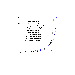
\includegraphics[width=0.55\textwidth]{images/chen-fin.eps}
\end{figure}
\vspace{-10pt}
    Еффективна проникність для двох зразків $\rm Ag-KCl$ (круги й трикутники) до порога перколяції та їх обробка згідно нашої теорії: $\varepsilon_0 = 5.0$, $\delta = 0.194$, $s = 0.72$ (чорна); $\varepsilon_0 = 7.0$, $\delta = 0.150$, $s = 0.74$ (синя). Середній радіус частинок $\rm Ag$: $R\approx 10$~нм. Вимірювана товщина оболонки: $\delta \approx 0.1$.
\end{frame}
%}
%%%%%%%%%%%%%%%%%%%%%%%%%%%%%%%%%%%%%%%%%%%%%%%%%%%%%
%{\setbeamertemplate{frame footer}{Експеримент: [I.-G. Chen, W. Johnson, J. Mat. Sci. {\bf 21} (1986) 3162]}
\begin{frame}{Порівняння з експериментальними даними з провідності}
\scriptsize{Експеримент: [I.-G. Chen, W. Johnson, J. Mat. Sci. {\bf 21} (1986) 3162]}
\footnotesize

\begin{figure}[tb]
    \centering
    \includegraphics[width=0.55\textwidth]{images/grannan-sigma-fin.eps}
\end{figure}
Ефективний опір зразку композита $\rm Ag-KCl$ (квадрати) та їх обробка згідно нашої теорії:
$\sigma_0 \approx 3.15 \times 10^{-8}$~С/м; $\sigma_1 \approx 6.3 10^7$~С/м; $\sigma_2 \approx 0.3 \times 10^3$~С/м; $\delta = 0.1682$ ($c_c = 0.214$).

\end{frame}
%}
%%%%%%%%%%%%%%%%%%%%%%%%%%%%%%%%%%%%%%%%%%%%%%%%%%%%%%%%%%%%%%%%%%%%%%%%%%%%%%%%%%%%%%%%%%%
\section{Аналіз диференціального підходу моделювання мікроструктури}%%%%%%%%%%%%%%%%%%%%%%%%%%%%%%%
%%%%%%%%%%%%%%%%%%%%%%%%%%%%%%%%%%%%%%%%%%%%%%%%%%%%%%%%%%%%%%%%%%%%%%%%%%%%%%%%%%%%%%%%%%

\begin{frame}{Диференціальна схема моделювання мікроструктури}
\footnotesize

Розглянемо систему твердих діелектричних куль в діелектричній матриці при деякій концентрації $c$ та ефективній проникності $\varepsilon$.

Моделювання $\delta\varepsilon$ в рамках {\bf МКГ (симетричного підходу)}:
\begin{equation}
    \delta\varepsilon_{\rm CGA} = (\varepsilon_0 - \varepsilon)[1 - \Pi_1] + (\varepsilon_1 - \varepsilon)\Pi_1 \Rightarrow 
    (1-c)\frac{\varepsilon_0 - \varepsilon}{2\varepsilon + \varepsilon_0} + c \frac{\varepsilon_1 - \varepsilon}{2\varepsilon + \varepsilon_1} = 0
\end{equation}

Моделювання в рамках {\bf асиметричного підходу Бругемана (АМБ)}:
\begin{eqnarray*}
    \delta\varepsilon_{\rm ABM}^{(l)} = (\varepsilon - (\varepsilon + \Delta\varepsilon))[1 - \Pi_1 - \Delta\Pi_1] 
    + (\varepsilon_1 - (\varepsilon + \Delta\varepsilon))\Delta\Pi_1 \\
    \approx -\Delta\varepsilon [1 - \Pi_1] + (\varepsilon_1 - \varepsilon) \Delta\Pi_1;
\end{eqnarray*}
\vspace{-5pt}
\begin{equation}
    - (1-c) \frac{\Delta \varepsilon}{3\varepsilon} + \Delta c \frac{\varepsilon_1 - \varepsilon}{2\varepsilon + \varepsilon_1} = 0
      \quad \Rightarrow \quad
      1 - c = \frac{\varepsilon - \varepsilon_1}{\varepsilon_0 - \varepsilon_1} \left( \frac{{ \varepsilon_0}}{\varepsilon} \right)^{1/3}.
\end{equation}


\begin{wrapfigure}{r}{0.4\textwidth}
\vspace{-20pt}
  \begin{center}
    \begin{overpic}[width=0.42\textwidth]{images/hanai-fig1.eps}
         %\put(60,70){$\rm KCl/Ag$}
    \end{overpic}
  \end{center}
%\vspace{-25pt}
\end{wrapfigure}

При зміні концентрації матриці:
$$
    \delta\varepsilon_{\rm ABM}^{(h)} \approx -\Delta\varepsilon \Pi_1 - (\varepsilon_0 - \varepsilon)\Delta\Pi_1;
$$
\begin{equation}
    c = \frac{\varepsilon - \varepsilon_0}{\varepsilon_1 + \varepsilon_0} \left( \frac{\varepsilon_1}{\varepsilon} \right)^{1/3}.
\end{equation}

\textbf{Електродинамічна взаємодія між новими порціями частинок та старими виконується за рахунок поточного ефективного середовища.}

\end{frame}
%%%%%%%%%%%%%%%%%%%%%%%%%%%%%%%%%%%%%%%%%%%%%%%%%%%%%
\begin{frame}{Побудова диференціальної схеми в рамках МКГ}
\footnotesize

Припущення: додавання інфінітизимальних порцій включень призводять до інфінітиземальних змін $c$ та $\varepsilon$.
\begin{equation}\label{eq:delta-Brug-diff0}
\begin{split}
  \widetilde{\delta\varepsilon}_{\rm CGA} ({\bf r}) = (\varepsilon_0 - (\varepsilon + \Delta\varepsilon)) [1 - ({\Pi}_1 ({\bf r}) + \Delta{\Pi}_1 ({\bf r}))]\\
  + (\varepsilon_1 - (\varepsilon +   \Delta\varepsilon)) [{\Pi}_1 ({\bf r}) + \Delta{\Pi}_1 ({\bf r})]
\end{split}
\end{equation}

Можна показати, що в загальному випадку, \textbf{локальне значення проникності буде формуватися за рахунок не тільки низько- та високо-концентраційних асиметричних вкладів, а ще й за рахунок частинок, що додавалися раніше}:
\begin{equation}
  \widetilde{\delta\varepsilon}_{\rm CGA} ({\bf r}) = \delta\varepsilon_{\rm ABM}^{(l)} ({\bf r}) + \delta\varepsilon_{\rm ABM}^{(h)} ({\bf r}) + \delta\varepsilon_{\rm CGA} ({\bf r}) \Rightarrow
\end{equation}
%що веде до диференціального рівняння:
$$
  \left[ \frac{\varepsilon_1 - \varepsilon}{2\varepsilon + \varepsilon_1} d c - (1 - c) \, \frac{3\varepsilon_0}{(2\varepsilon + \varepsilon_0)^2} d\varepsilon \right] 
  + \left[ - \frac{\varepsilon_0 - \varepsilon}{2\varepsilon + \varepsilon_0} d c
  - c \, \frac{3\varepsilon_1}{(2\varepsilon + \varepsilon_1)^2} d\varepsilon \right] = 0.
$$

\end{frame}
%%%%%%%%%%%%%%%%%%%%%%%%%%%%%%%%%%%%%%%%%%%%%%%%%%%%%
\begin{frame}{Аналіз результату}
\footnotesize

При переході до низько- та високо-концентраційних крім вкладу АМБ присутні вклади частинок, що додавалися раніше.

  \metroset{block=fill}
  \begin{block}{Низькоконцентраційна межа}
    \begin{equation}
        \widetilde{\delta\varepsilon}_{\rm CGA}^{(l)} \approx \delta\varepsilon_{\rm ABM}^{(l)} + \delta\varepsilon_{\rm CGA} \Rightarrow
        \frac{d c}{1-c} = d\varepsilon \frac{3\varepsilon_0(2\varepsilon + \varepsilon_1)}{(\varepsilon_1 - \varepsilon) (2\varepsilon + \varepsilon_0)^2}
    \end{equation}
    \begin{eqnarray}\label{eq:Hanai-new}
        \ln{(1-c)} = \frac{9 \varepsilon_0 \varepsilon_1}{(2\varepsilon_1 + \varepsilon_0)^2} \ln{\left[ \frac{3\varepsilon_0 (\varepsilon - \varepsilon_1)}{(\varepsilon_0 - \varepsilon_1) (2\varepsilon + \varepsilon_0)} \right]} 
        - \frac{2(\varepsilon_0 - \varepsilon_1) (\varepsilon_0 - \varepsilon)}{(2\varepsilon_1 + \varepsilon_0) (2\varepsilon + \varepsilon_0)}
    \end{eqnarray}
  \end{block}
  
  \begin{block}{Висококонцентраційна межа}
    \begin{equation}
        \widetilde{\delta\varepsilon}_{\rm CGA}^{(h)} \approx \delta\varepsilon_{\rm ABM}^{(h)} + \delta\varepsilon_{\rm CGA} \Rightarrow
        \frac{d c}{c} = - d\varepsilon \frac{3\varepsilon_1 (2\varepsilon + \varepsilon_0)}{(\varepsilon_0 - \varepsilon) (2\varepsilon + \varepsilon_1)^2}
    \end{equation}
    \begin{eqnarray}
        \ln{c} = \frac{9 \varepsilon_0 \varepsilon_1}{(2\varepsilon_0 + \varepsilon_1)^2} \ln{\left[ \frac{3\varepsilon_1 (\varepsilon - \varepsilon_0)}{(\varepsilon_1 - \varepsilon_0) (2\varepsilon + \varepsilon_1)} \right]} 
        - \frac{2(\varepsilon_1 - \varepsilon_0) (\varepsilon_1 - \varepsilon)}{(2\varepsilon_0 + \varepsilon_1) (2\varepsilon + \varepsilon_1)}
    \label{eq:Hanai-high-new}
    \end{eqnarray}
  \end{block}
  
  \textbf{$\delta\varepsilon_{\rm CGA}$ можна знехтувати якщо: 1) $\varepsilon_0 \approx \varepsilon$ та $\varepsilon_1 \approx \varepsilon$; 2) концентрації, що додаються досить малі; 3) $|\varepsilon_1-\varepsilon_0|$ також мале.}


\end{frame}
%%%%%%%%%%%%%%%%%%%%%%%%%%%%%%%%%%%%%%%%%%%%%%%%%%%%%
\begin{frame}{Порівняння результатів з границями Хашина-Штрікмана}

\begin{figure}[tb]
    \centering
    \includegraphics[width=0.55\textwidth]{images/hanai-fig2.eps}
    \caption{\label{fig:HSbounds}
    Концентраційна залежність $\varepsilon$ згідно з: отриманими низько- та високо-концентраційними залежностями в рамках МКГ (товсті чорні лінії 1, 2, відповідно); нижня та верхня границі Хашина-Штрікмана (тонкі лінії 3 та 4); підхід МКГ (штрихована лінія); оригінальні низько- та високо-концентраційні асиметричні підходи Бругемана (точкові лінії 5 та 6). При побудові був використаний тільки один параметр $\varepsilon_1/\varepsilon_0 = 10^2$.}
\end{figure}

\end{frame}


%%%%%%%%%%%%%%%%%%%%%%%%%%%%%%%%%%%%%%%%%%%
%\section{Висновки}%%%%%%%%%%%%%%%%%%%%%%%%%
%%%%%%%%%%%%%%%%%%%%%%%%%%%%%%%%%%%%%%%%%%%

\begin{frame}{Висновки}

--- В рамках методу компактних груп неоднорідностей побудована послідовна статистична модель макроскопічно однорідної та ізотропної дисперсної системи з морфологією частинок типу тверде ядро--проникна оболонка у довгохвильовом наближенні.\vspace{10pt}

--- Згідно з результатами тестування на даних числових симуляцій RRN, теорія адекватно описує концентраційну поведінку статичної провідності систем з електрично однорідними та неоднорідними оболонками.\vspace{10pt}

--- Результати обробки експериментальних даних з $\sigma_{\rm eff}$ систем композитних електролітів наведеною теорією свідчать про вплив на $\sigma_{\rm eff}$ обох вкладів: високопровідних оболонок та зміни провідності матриці.

\end{frame}
%%%%%%%%%%%%%%%%%%%%%%%%%%%%%%%%%%%%%%%%%%%%%%%%%%%%%
\begin{frame}{Висновки}

--- Аналіз перколяційної поведінки провідності та проникності в рамках теорії показав, що поріг перколяції залежить лише від геометричних властивостей системи; критичні індекси перколяції, що вимірюються на експерименті, носять не універсальний характер, а залежать від концентраційної області їх вимірювання.\vspace{10pt}

--- Порівняння результатів обробок розглядуваних систем наведеної теорії з підходами Максвела-Гарнета, Бругемана та Накамури-Нана свідчать про істотну гнучкість першої.\vspace{10pt}

--- Аналіз диференціальної схеми в рамках теорії показав її загальну непослідовність для розглядуваних систем в довгохвильовому наближенні.

\end{frame}



%%%%%%%%%%%%%%%%%%%%%%%%%%%%%%%%%%%%%%%%%%%%%%%%%%%%%
{\setbeamercolor{palette primary}{fg=black, bg=white}
\begin{frame}[standout]
  Дякую за увагу!
\end{frame}
}



\end{document}
